\subsection{Reliability Computation}
In this section, we compare the approaches for computing the travel
time distribution based on link travel time predictions for a given path,
discussed in Section \ref{sec:methods}. The approaches have different
characteristics regarding
\begin{itemize}
  \item link travel time representation: discrete (Dis) or continuous (Con),
  i.e., through a normal distribution.
  \item time-dependency: consideration of time-dependency (Tim) or static (Sta)
  interpretation.
  \item correlation: consideration of correlation (Cor) or assumption of
  independence (Ind) between link travel time.
\end{itemize}

Accordingly, we use this naming scheme for the approaches DisStaInd and
ConStaInd (discussed in Section \ref{subsec:static}), DisTimInd (discussed
in Section \ref{subsec:time}), DisStaCor and ConStaCor (discussed
in Section \ref{subsec:cor}) and DisTimCor (discussed
in Section \ref{subsec:timcor}).

In this section, we use 5 different paths, spanning the road network in \ref{subsec:Dataset}. The selected
paths are 45 miles on average, consisting of approximately 40 edges. For each
path, we use the same standard \textit{start times} we used for the link travel time predictions. Again, we build a model with each approach using data from model days and compare the accuracy of the model with the actual travel time during the test days.

\begin{figure}[h]
	\centering
	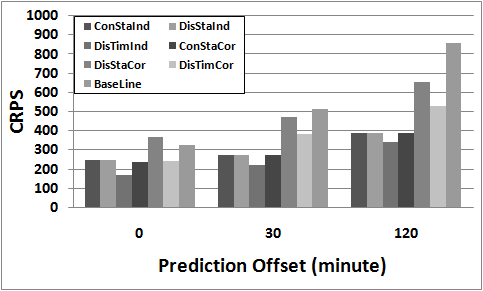
\includegraphics[width = 0.75\columnwidth]{figures/path1_results.png}
	\caption{CRPS for probabilistic path computation}\label{fig:path_comp}
		\vspace{-0.3cm}
\end{figure}

The results comparing all approaches are shown in Figure \ref{fig:path_comp}.
The \textit{prediction offset} in this scenario is the time between the
\textit{query time} and the \textit{start time} of the whole route (i.e., the
\textit{prediction offset} for a single link on the route may be larger in the
time-dependent approaches). Several observations can be derived from this
experiment:

Comparing ConStaInd and DisStaInd, we can observe the same characteristics than
for single links. Representing the link travel times trough a \textit{pmf} or a
normal distribution do not drastically change the accuracy of the travel time
prediction.

Incorporating the time variablity of the network (DisTimInd) however, has a very
positive effect on the prediction accuracy, where the results are up to 25\%
better compared to the time-independent approaches which have otherwise the same
characteristics.

The ConStaCor approach is again time-independent and it seems that the
consideration of correlation between links does only yield a marginal
improvement over the same approach without correlation (ConStaInd). In our
experiments, we observe only a 1\%-2\% improvement through the incorporation of
correlation in this setting.

The consideration of correlation in the discrete approaches (DisStaCor and
DisTimCor) has even a negative effect on the prediction quality. This is due to
the fact that correlation here is incorporated in a completely different way
than in the continuous case. In our opinion, the aggravation of these approaches
compared to their counterparts without correlation (DisStaInd and
DisTimInd) may have three reasons. First, the modelling of correlation
through the two states (congested/non-congested) is inadequate to capture the
correlation between consecutive links. Second, the realization of the two states
as proposed by us could be inadequate. Last, the correlation is computed over
the whole dataset and thus represents a global relation. Maybe better results
could be achieved if the correlation was time-dependent too.

As an additional comparison partner we included an approach that is used in
current route planing systems, named \textit{Baseline}. \textit{Baseline}
uses the situation at the \textit{query time} and computes the path travel time
without prediction based on the currently available deterministic travel times. The
outcome will consequently be a non-probabilistic value as well. The CRPS method allows
us to directly compare this approach to the probabilistic counterparts, since it
converges to the mean error in the case of certain predictions (i.e., the CRPS
can be interpreted as the difference of the prediction and the true value in
seconds). The results show that under all settings (with DisStaCor with 0
prediction offset being an exception) the probabilistic approaches are superior
to the \textit{Baseline} approach which once more justifies the use of
probabilistic models in this application.


\begin{figure}[h]
	\centering
	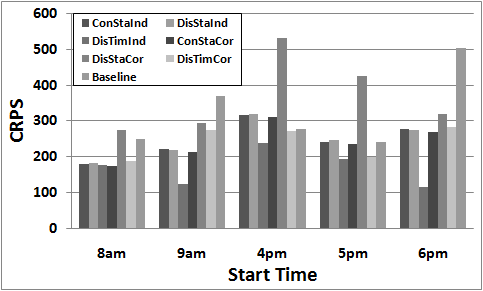
\includegraphics[width = 0.7\columnwidth]{figures/path2_results.png}
	\caption{CRPS for different start times}\label{fig:path_comp2}
	\vspace{-0.3cm}
\end{figure}

Figure \ref{fig:path_comp2} shows the above results for \textit{prediction
offset} = 0 and broken down into different \textit{start times}. The overall
effects are similar. However, it is worth noting that the performance of the
approaches is indeed dependent on the \textit{start time}. E.g., the
time-dependent approaches yield a much better result compared to the other
methods at 9:00am and 6:00pm, which is as expected since these are the times in
metropolitan road networks at which the traffic usually starts getting much better than
in the two hours before, thus we expect a lot of changes in the travel times of
single links around these times.

\begin{figure}[h]
	\centering
	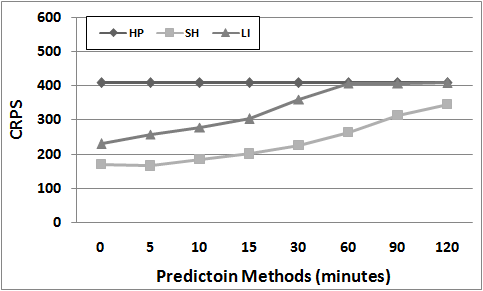
\includegraphics[width = 0.75\columnwidth]{figures/DTI_results.png}
	\caption{CRPS of DisTimInd for different prediction
	methods}\label{fig:dti_results}
\end{figure}

\begin{figure}
    \centering
    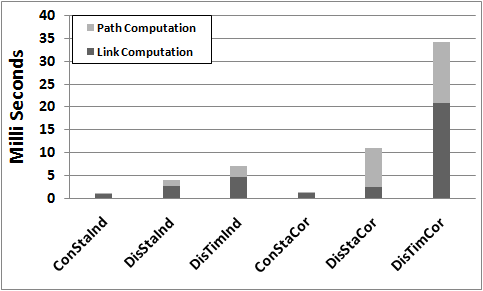
\includegraphics[width = 0.75\columnwidth]{figures/runTime_results.png}
    \caption{Runtimes}\label{fig:runtimes}
\end{figure}

In order to evaluate the effect of the other link prediction methods we tested
all three of them as the basis for the DisTimInd approach (cf Figure
\ref{fig:dti_results}). The results reflect the results on the single link
prediction and are consistent across all path travel time computation methods.
Again, SH is the prediction method that yields the best prediction accuracy.

Lastly, we evaluated the runtime of all path computation methods discussed in
Section \ref{sec:methods}. Runtimes are broken into link travel time
prediction and path computation in Figure \ref{fig:runtimes}. Generally, the
continuous approaches perform much better due to the analytical nature which
yields a much better runtime complexity. As expected, the more complexity we add
to the approaches based on a discrete representation, the more costly in terms
of computation they become, whereupon considering correlation adds most of the
complexity. Link travel time prediction and path computation contribute rather
equivalent portions to the runtime in all approaches.


